\documentclass[12pt]{article}
\usepackage{fullpage}
\usepackage{amsmath,amssymb,mathtools,xparse,graphicx,float,datetime,color,array,graphics,enumerate,tikz,pgfplots,xcolor}
\usepgfplotslibrary{statistics}
\pagestyle{empty}
\newcommand{\D}{\displaystyle}
\setlength{\textheight}{9in} \setlength{\headheight}{.2in}
\setlength{\headsep}{0in} \setlength{\topmargin}{0in}
\begin{document}
\begin{center}
CSCI 6100 Machine Learning From Data\\
Fall 2018\\
\end{center}
\begin{center}
HOMEWORK 5\\
Daniel Southwick\\
661542908\\
southd@rpi.edu
\end{center}
\vspace{.1in}

\noindent {\bf Exercise 2.8} \\\\
\indent a) Consider generating $K$ data sets $\mathcal{D}_1,...,\mathcal{D}_k$ and apply the learning algorithm to each data set to produce hypothesis $g_1,...,g_k$, then $\displaystyle \bar{g} = \frac{1}{K}\sum_{k=1}^{K}g_k(\textbf{x}) = \frac{1}{K}g_1+\frac{1}{K}g_2+\dots+\frac{1}{K}g_k$. And since $g_i$ is in the hypothesis set $\mathcal{H}$, $\forall i \in {1,...,K}$, and the set is closed under linear combination, so $\displaystyle\frac{1}{K}\sum_{k=1}^{K}g_k(\textbf{x})$ is in the set $\mathcal{H}$ as well. Thus $\bar{g} \in \mathcal{H}$.\\\\
\indent b) Consider a binary target function, such that $\mathcal{H}$ only contains two hypothesis: $\{+1,-1\}$. So if the final hypothesis is $+1$ fir sine data sets, and $-1$ for other data sets. Then for any $x$, $\displaystyle bar{g}(x) = \frac{1}{K}\sum_{k=1}^{K}g_i(x) \in (-1,+1)$, thus $\bar{g} \not \in \mathcal{H}$.\\\\
\indent c) No, Consider $g_1(\textbf{x}) = 
			\left\lbrace \begin{array}{ll}
			-1 & x < 0 \\
			+1 & x> 0
			\end{array}\right.$
			and 
			$g_2(\textbf{x}) = 
			\left\lbrace \begin{array}{ll}
			+1 & x < 0 \\
			-1 & x> 0
			\end{array}\right.$, which are both binary functions. But then $\bar{g}(x) = 0$ for all $x$, the average function is not a binary function.\\\\
			
\noindent {\bf Problem 2.14} \\\\
\indent a) Since the VC dimension of $\mathcal{H}_i$ is $d_{vc}$, $\forall i \in \{ 1,...,K\}$, when break point $k = d_vc + 1$, then no data set of size $k$ can be shattered by $\mathcal{H}_i$, $\forall i \in \{1,...,K\}$. So, as $\mathcal{H} = \mathcal{H}_1 \cup ... \cup \mathcal{H}_K$, the overall possible dichotomies for the hypothesis $\mathcal{H} < (2^{dvc+1})^K = 2^{K(dvc+1)}$. Since $k_{H} = d_{vc}(H) + 1$, then $d_{vc}(\mathcal{H}) < K(d_{vc} + 1)$.\\\\
\indent b)Since $m_{\mathcal{H}}(N) \leq N^{d_{vc}}+1 $, then, $m_{\mathcal{H}_i}(l) \leq l^{d_{vc}}+1,\ 1\leq i \leq K$ and based on (2.10), we know that $m_{\mathcal{H}}(l) \leq l^{d_{vc}}+1$, thus $m_{\mathcal{H}}(l) \leq Kl^{d_{vc}}+K$. And since $\mathcal{H} = \mathcal{H}_1\cup\mathcal{H}_2\cup\dots\cup\mathcal{H}_K$, we have $m_{\mathcal{H}}(l) \leq K(l^{d_{vc}}+1)\leq 2Kl^{d_{vc}} \leq 2l$, thus $d_{vc}(\mathcal{H}) \leq l$\\\\
\indent c) Since we need to prove that $d_{vc}(\mathcal{H})\leq \min( K(d_{vc}+1), 7(d_{vc}+K)\log_2(d_{vc}K))$, we can plug in the result, $d_{vc}(\mathcal{H}) < K(d_{vc}+1)$ from a) into b) with the term $l = 7(d_{vc}+K)\log_2(d_{vc}K)$. Then we can show that $2^l > 2Kl^{d_{vc}}$. So $d_{vc}(\mathcal{H})\leq \min( K(d_{vc}+1), 7(d_{vc}+K)\log_2(d_{vc}K) )$.\\\\

\newpage
\noindent {\bf Problem 2.15} \\\\
\indent a) \begin{figure}[H]
  \centering
  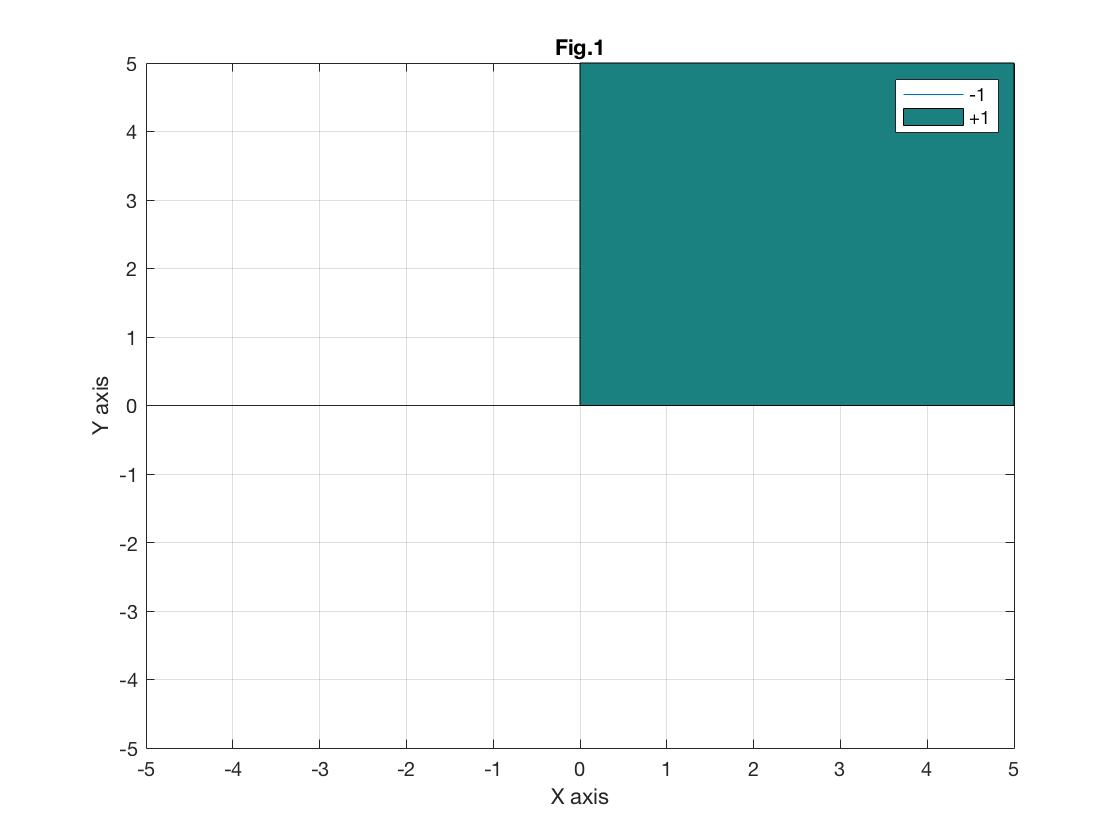
\includegraphics[scale = 0.35]{Pic1.jpg}
  \caption{Example of a 2D monotonic classifier}
  \label{fig:Pic1}
\end{figure}
\indent If $x$ lies in the first quadrant then $h(x) = +1$, otherwise, $h(x) = -1$.\\\\
\indent b) From the hint, Consider a set of $N$ points generated by first choosing one point and, then generating the next point by increasing the first component and decreasing the second component until $N$ points are obtained. So no matter $x_i = +1 or -1$, $x_{i+1}$ are also $+1$ or $-1$. So given N points, the number of all possible dichotomies is $m(H) = 2^N$, Thus $d_{vc} = \infty$\\\\

\noindent {\bf Problem 2.24} \\\\
\indent a) From the data set $\{ (x_1,x_1^2),(x_2,x_2^2) \}$, we can obtain the linear function: \begin{center}$\displaystyle g(x) = x_1^2 + \frac{x_2^2-x_1^2}{x_2-x_1}(x-x_1) = (x_1+x_2)x - x_1x_2$ \end{center} Therefore, the average function is \begin{center} $\displaystyle \bar{g}(x) = \mathbb{E}_{\mathcal{D}}(g^{\mathcal{D}}(x))$\\$= \frac{1}{2}\times\frac{1}{2}\int_{-1}^{1}\left(\int_{-1}^{1}\left[(x_1+x_2)x-x_1x_2\right]\ \mathrm{d}x_1\right)\ \mathrm{d}x_2$\\$=0$\end{center}
\indent \indent b) We first generate the test dataset with 2000 items selected uniformly from the interval [-1,+1] and compute $f(x)$. Then for 1000 times, we choose two numbers $x_1,x_2$ randomly from [-1,+1] again, and determine the linear function $g$ given $\{ (x_1,x_1^2),(x_2,x_2^2) \}$.  Then we calculate: \begin{align*}\displaystyle
			\mathsf{bias} &= \mathbb{E}_x( \bar{g}(x)-f(x) )^2 = \frac{1}{2}\int_{-1}^{1}( \bar{g}(x)-f(x) )^2\ \mathrm{d}x \\
			\mathsf{var} &= \mathbb{E}_{\mathcal{D}}[ g^{\mathcal{D}}(x)^2] - \bar{g}(x)^2= \frac{1}{2}\int_{-1}^{1}\left[ \frac{1}{K}\sum_{k = 1}^K (g_k(x)-\bar{g}(x))^2\ \right]\mathrm{d}x \\
			\mathsf{E_{out}} 
			& = \mathbb{E}_{x}\left[\mathbb{E}_{\mathcal{D}}[(g^{(\mathcal{D})}(x)-f(x))^2]\right] = \frac{1}{2}\int_{-1}^{1} \left[\ \frac{1}{K}\sum_{k = 1}^K (g_k(x)-f(x))^2\ \right] \mathrm{d}x
		\end{align*}
\indent c) In the stimulation, we used 2000 points from [-1,+1] and run through 1000 times for different g's the end average function is: \begin{center} $g(x) = -0.0031884x + 0.0019613$\end{center} With $\mathsf{bias} = 0.18653$, $\mathsf{variance} = 0.31428$ and $\mathsf{E_{out}} = 0.52038$. Note that $\mathsf{E_{out}} \approx \mathsf{bias}+\mathsf{variance}$. Result from Matlab:\begin{figure}[H]
  \centering
  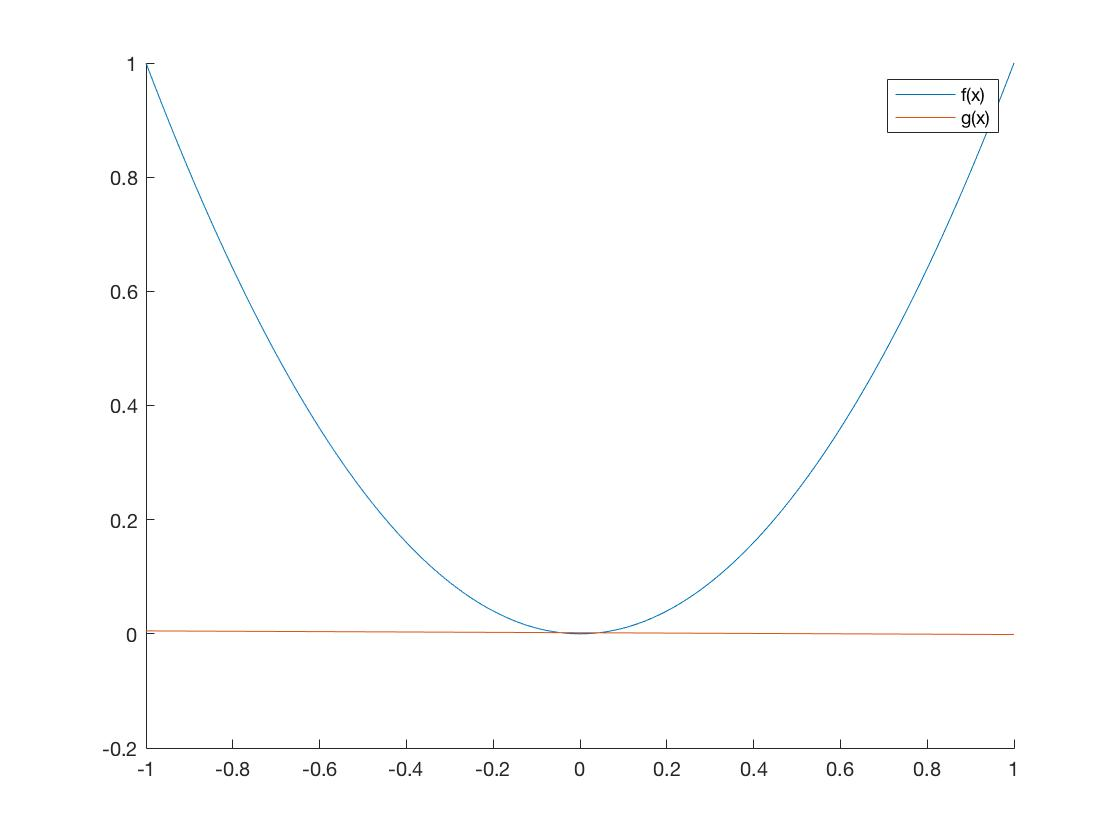
\includegraphics[scale = 0.35]{Pic2.jpg}
  \caption{f(x) and g(x)}
  \label{fig:Pic2}
\end{figure}
\indent \indent d) \begin{center} 
$\displaystyle \mathsf{bias} = \mathbb{E}_x( \bar{g}(x)-f(x) )^2 = \frac{1}{2}\int_{-1}^{1}( \bar{g}(x)-f(x) )^2\ \mathrm{d}x$\\
$\displaystyle = \frac{1}{2} \int_{-1}^{1}(x^2)^2\ \mathrm{d}x$\\
$\displaystyle =0.2$\\ \indent \\\indent \\
$\displaystyle \mathsf{var} = \mathbb{E}_{\mathcal{D}}[ g^{\mathcal{D}}(x)^2] - \bar{g}(x)^2= \frac{1}{2}\int_{-1}^{1}\left[ \frac{1}{K}\sum_{k = 1}^K (g_k(x)-\bar{g}(x))^2\ \right]\mathrm{d}x$\\
$\displaystyle = \frac{1}{2}\times\frac{1}{2}\int_{-1}^{1}\left(\int_{-1}^{1}(\left[(x_1+x_2)x-x_1x_2\right]-0)^2\ \mathrm{d}x_1\right)\ \mathrm{d}x_2$\\
$\displaystyle = \frac{1}{4}\times\frac{4}{9}(6x^2+1) = \frac{1}{9}(6x^2+1) = \frac{2}{3} x^2 + \frac{1}{9}$\\
$\displaystyle = \frac{1}{2} \int_{-1}^{1}(\frac{2}{3}x^2+\frac{1}{9})^2\ \mathrm{d}x$\\
$\displaystyle = \frac{1}{3}$\\ \indent \\\indent \\
$\displaystyle \mathbb{E}_{x} =  \mathsf{bias} + \mathsf{var} = \frac{1}{5} + \frac{1}{3} = \frac{8}{15}$

\end{center}

\end{document}
